
\section{Introduction}
A reproducible setup environment needs to be established in order to maximize the software's potential to reduce energy consumption.

This chapter will be devoted to giving a set of guidelines with the intention of delivering a test that is accurate, representative, and replicable.

% This chapter will go over each component in further detail, describe it, and explain how it is used in the field of empirical analysis for software energy optimization.

\section{Threats and Challenges}

A successful benchmark must meet three criteria.
First, it must be \textbf{reproducible} in order for others to imitate it.
Second, the findings should be \textbf{accurate},which implies that we should expect the same results each time we run the benchmark.
Finally, it should \textbf{represent} reality.
In other words, the experiment's findings should be applicable outside of the research lab as well.
The aim of \textbf{representativeness} in this thesis is the manufacturing environment.
As a result, the experiments should reflect what happens in production contexts.


%%%%%%%%% preliminary taughts and section structure 
% The need of reproducibility in our field - software optimization based on empirical studies -

% The importance of Virtualisation for reproducibility \cite{howe_virtual_2012}
% some of the most important parts are
% - fewer constraints on research methods
% - on-demand backups
% - virtual Machines as Publications
% - more Variables captured

\subsection{Reproducibility}
The reproducibility of experiments is often ranked as one of the most difficult difficulties faced by researchers. In point of fact, many of the outcomes cannot be duplicated.,\footnote{Trouble at the lab, The Economist, 19 October 2013;  www.economist.com/news/briefing/ 21588057-scientists-think-science-self-correcting- alarming-degree-it-not-trouble.} which led to a \emph{replication crisis}.
As this crisis hit most of the empirical studies, most of the reviews now includes reproducibility as one of the minimal standard for judging scientific merit.\cite{peng2011reproducible}
One of the criterions supporting reproducibility is the publication of the dataset and the algorithms run on the raw data to conclude the results.
There is even some disagreement about what the terms "reproducibility" or "replicability" by themselves mean \cite{goodman2016does}.
According to \cite{echtler2018open}, \emph{replicability} extends \emph{reproducibility} with the ability to collect a new raw dataset comparable to the original one by re-executing the experiment under similar condition, instead of just the ability to get the same results by running the statistical analyses on the original data set.

In the area covered by this PhD thesis, reproducibility might be achieved by ensuring the same execution settings of physical nodes, virtual machines, clusters or cloud environments.
However, when it comes to measuring the energy consumption of a system, applying acknowledged guidelines and carefully repeating the same benchmark can nonetheless lead to different energy footprints not only among homogeneous nodes, but even within a single node.

One major problem that hinders the reproducibility of the empirical benchmarks is the interaction with the external environment, either as concurrency or dependencies.
Therefore, researchers cannot observe the same results, unless they duplicate the same environment.


\subsection{Accuracy}
According to Oxford, \emph{accuracy} means \href{https://www.lexico.com/definition/accuracy}{"technical The degree to which the result of a measurement, calculation, or specification conforms to the correct value or a standard"}.
In ny case, this means the ability to run the benchmark multiple times with a low variation.

Recently, the research community has been investigating typical "crimes" in systems benchmarking and established guidelines for conducting robust and reproducible evaluations~\cite{DBLP:journals/corr/abs-1801-02381}.

In theory, using identical CPU, same memory configuration, similar storage and networking capabilities, should increase the accuracy of physical measurements.
Unfortunately, this is not possible when it comes to measuring the energy consumption of a system.
Applying the benchmarking guidelines and repeating the same experiment with in the same configuration are not sufficient to reproduce the the same energy measurements, not only between identical machines, but even within the same machine.
This difference---also called \emph{energy variation} (EV)---has become a serious threat to the accuracy of experimental evaluations.

Figure~\ref{fig:motivation} illustrates this variation problem as a violin plot of $20$ executions of the benchmark \emph{Conjugate Gradient} (\textsf{CG}) taken from the \emph{NAS Parallel Benchmarks} (NBP) suite~\cite{Bailey:1991:NPB:125826.125925}, on $4$ nodes of an homogeneous cluster (the cluster \textsf{Dahu} described in Table~\ref{table:g5k}) at 50\,\% workload.
We can observe a large variation of the energy consumption, not only among homogeneous nodes, but also at the scale of a single node, reaching up to $25\,\%$ in this example.

\begin{figure}%[!htb]
    \center{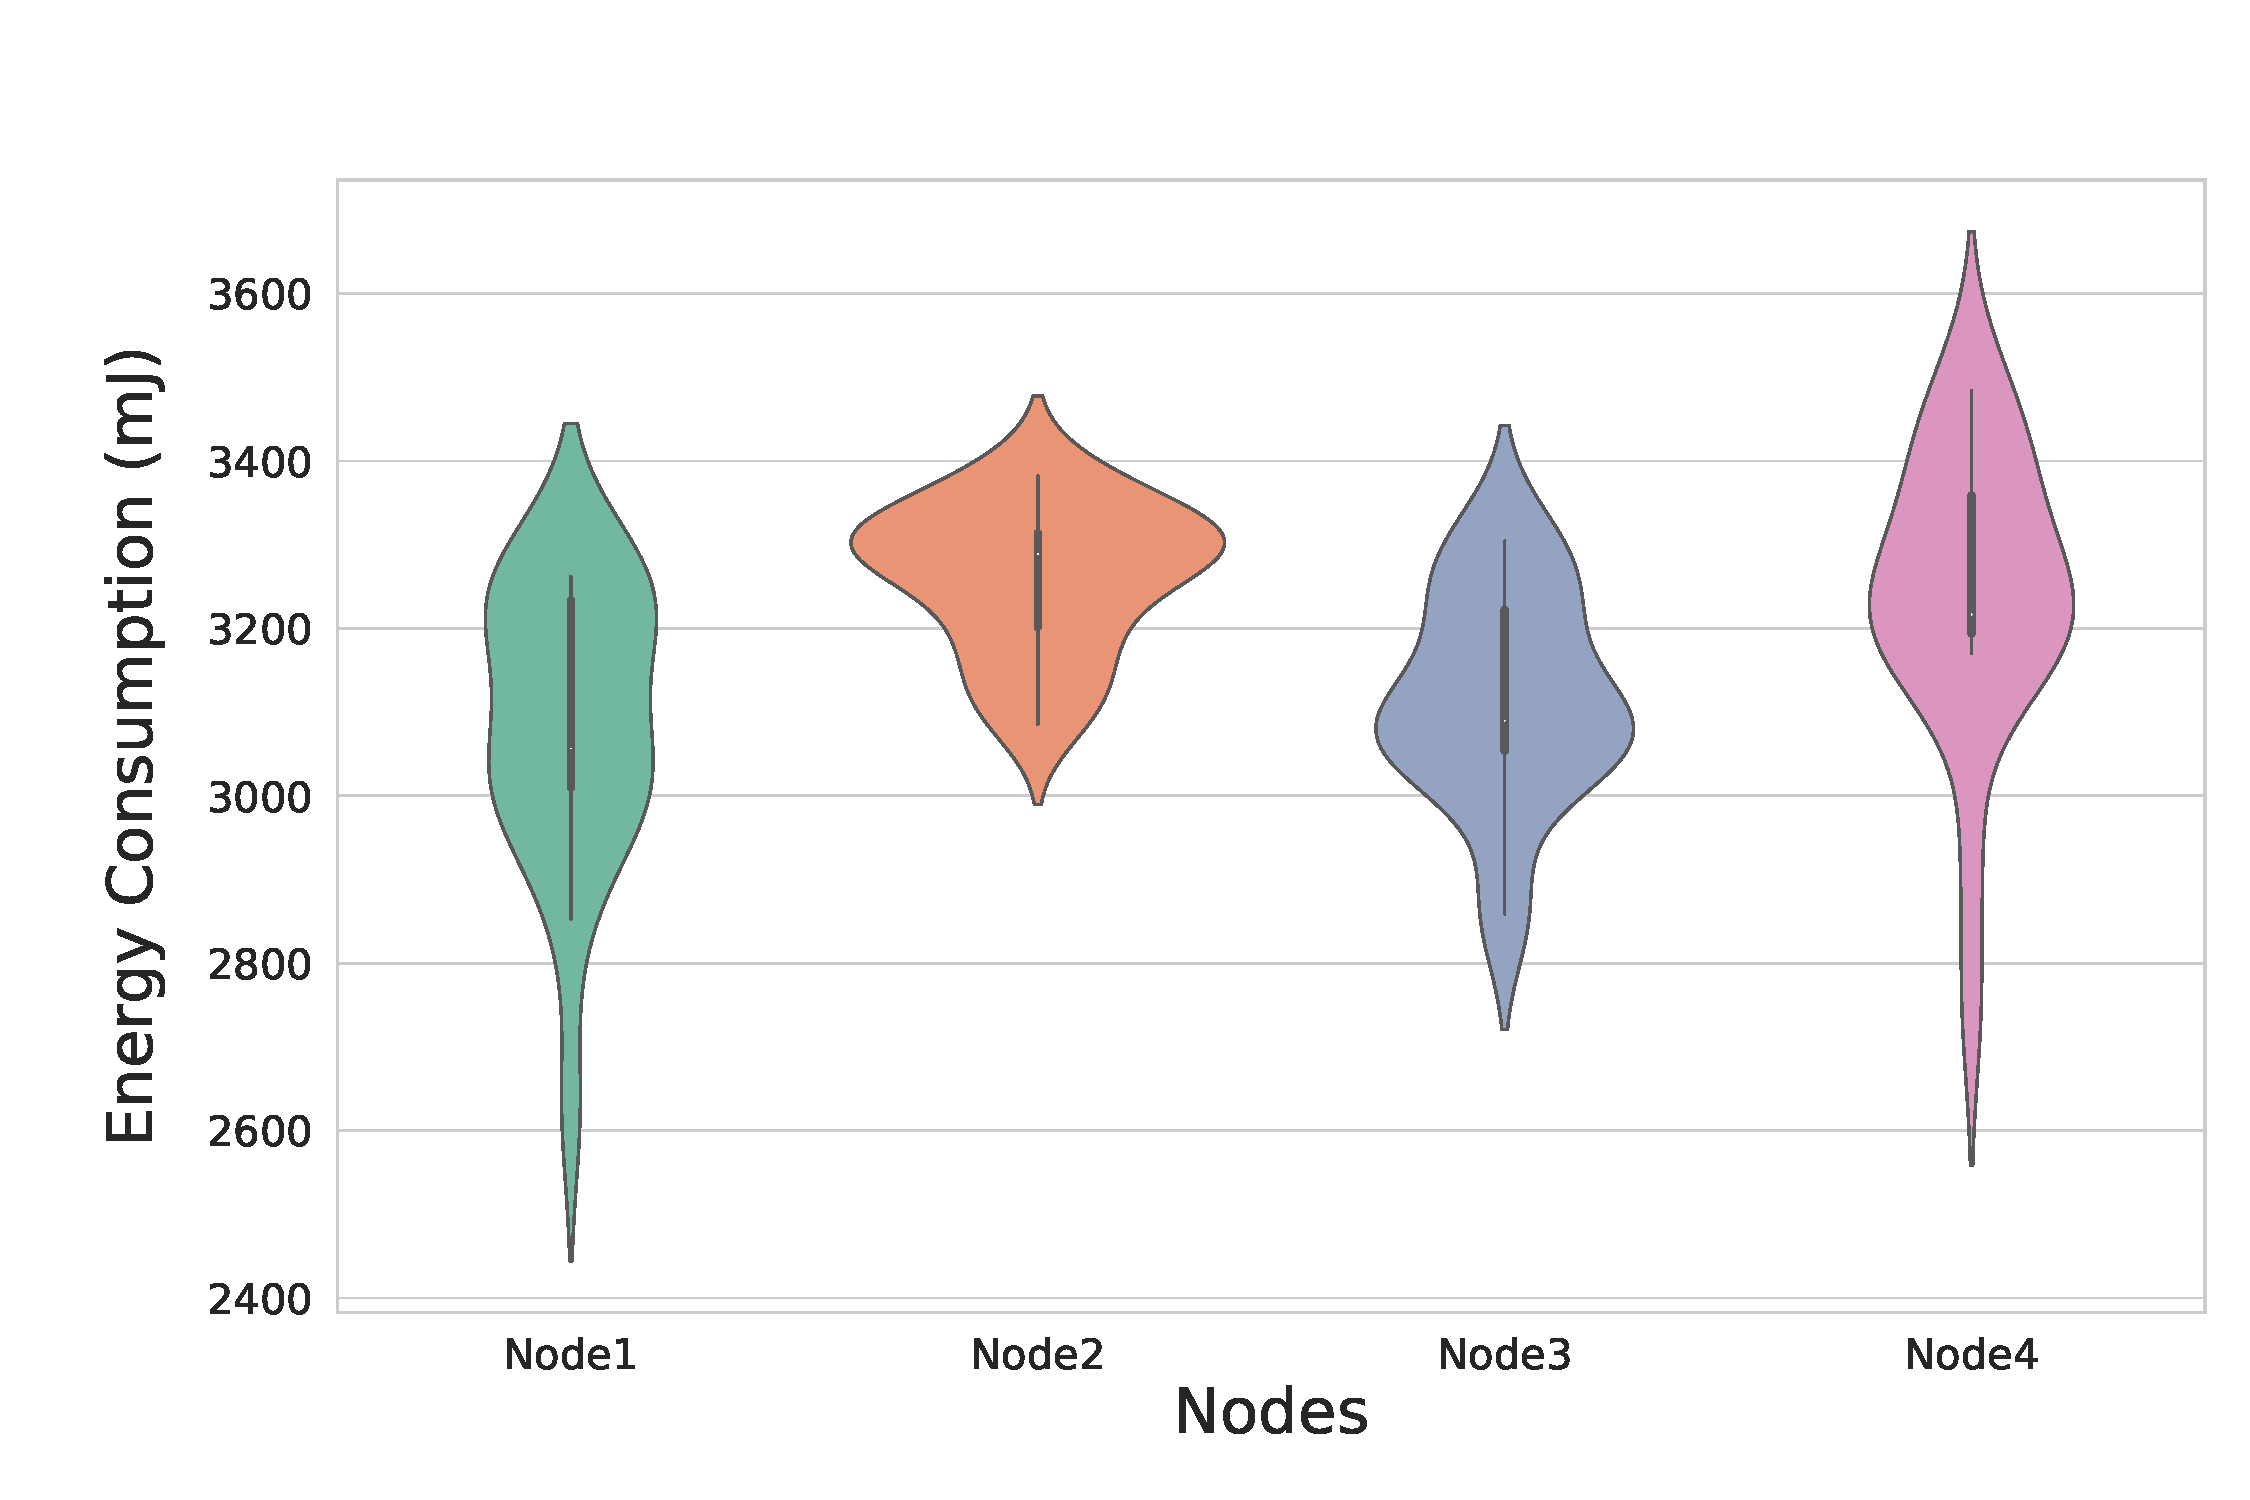
\includegraphics[width=.9\linewidth]{imgs/motivation}}
    \caption{CPU energy variation for the benchmark \textsf{CG}}\label{fig:motivation}
\end{figure}

Some researchers started investigating the hardware impact of the energy variation of power consumption.
As an example, one can cite~\cite{borkar_designing_2005,tschanz_adaptive_2002} who reported that the main cause of the variation of the power consumption between different machines is due to the \textbf{CMOS} manufacturing process of transistors in a chip.
\cite{heinrich_predicting} described this variation as a set of parameters, such as CPU Frequency and the thermal effect.


\subsection{Representativeness}
As obvious as it seems, the reason of executing benchmarks is to validate ideas so we can use them in the real life.
However, this is means that those benchmarks have to represent reality somehow.
Basically, when we aim to benchmark something, we create a mock up version of the situation that we want it to work.
% But, how can we assure that the benchmark is representative? honestly i don't know. and we can't generalize this. but there are some works that have been done for this.
First, we can talk about the benchmarking and their selection, then we will talk about the stress benchmark for some applications, and finally we will bring this representativeness in our case and how can we get closer to the energy consumption behavior of a software between the benchmark environnement and the production one.

As Stephen M. Blackburn~\emph{et~al.} cited in their paper "evaluate collaboratory"~\cite{stephen_evaluate_2012}, one of the major pitfalls of the measurement contexts is the inconsistency, which can be translated here by the fact that the production context is not the same as the benchmarking one.

Another difficult part for practitioners is to generalize the claims they reached beyond the lab conditions.
Are they appropriate?
Are they consistent and are they reproducible?
To answer those questions, the community agreed on some wellknown benchmarks to represent a specific concern of the production world.
One can site as an example the Dacapo and Renaissance benchmark suites for Java applications, or the CLBG benchmark suite for comparing programming languages.
Although they do not cover all the cases, the community agrees on their relevance and representativeness.


In addition to these benchmarks, a new category of testing techniques has emerged to simulate the worst cases of the production environments. This new category of benchmarking called performance tests\cite{pradeep2019pragmatic}, which are benchmarks meant to evaluate the behavior of software under stress situations. We can use the Gatling\footnote{\url{https://gatling.io/}} as an illustration for web applications stresser and stress-ng for hardware heavy workload perormance measurements~\cite{king2017stress}.

\subsection{Extension}
Morover, The field of computer science is seeing rapid advancements, which has led to an increase in the number of obsolete results. Even more so, when it comes to studies that compare multiple solutions, it is impossible to cover them all.
In addition, between the preliminary experiment and the results that were published, there may have been the appearance of new candidates as well as the development of others. As a result, we would like to provide a fresh idea for a productive experiment that we will call "Extension." The ability to give the required tools to not only repeat the experiment but also to add additional candidates, workloads, or key metrics.

\subsection{conclusion}


We propose making certain enhancements to the benchmarking framework that was suggested by the collaboratory on Experimental Evaluation of Software \footnote{\url{http://evaluate.inf.usi.ch/}}. and Systems in Computer Science in order to address those problems.
Instead of only presenting the four primary aspects of their guidelines, which are \emph{measurement contexts} that indicate the software and hardware components that will alter or remain constant during the experiment. \emph{workloads} which identify the benchmarks to use in the experiment, as well as their inputs; \emph{metrics} that specify the attributes to be measured and how to assess them. \emph{Data analysis} show how to examine data and evaluate the outcomes of the analysis to offer insight into the assertions that arise from the study.

\begin{itemize}
    \item \textbf{candidates}: a set of candidates that will be used in the experiment. The candidates should be agnostic of the experiment context and they all
\end{itemize}





\begin{figure}%[!htb]
    \center{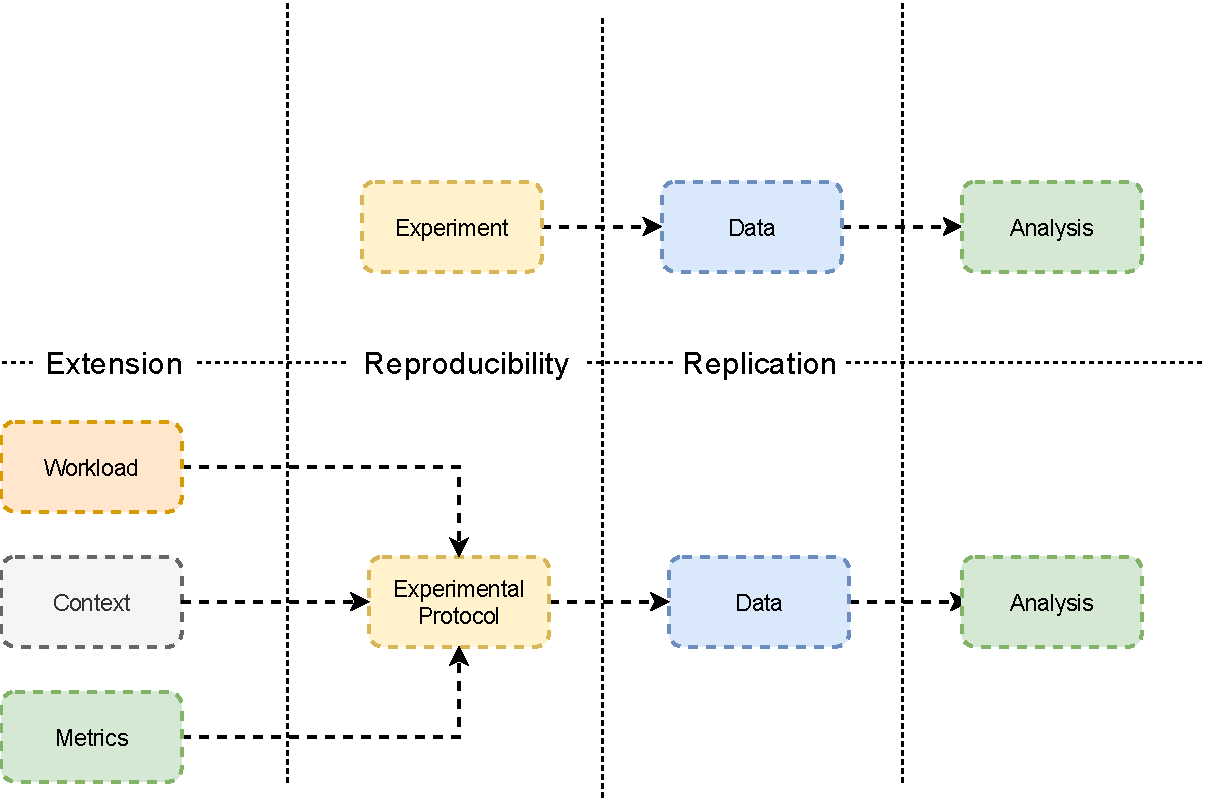
\includegraphics[width=.9\linewidth]{imgs/benchmarkingprotocol}}
    \caption{Benchmarking protocol}\label{fig:benchmarkingprotocol}
\end{figure}



% A more subtle issue may arise due to the values of the measurements that we achieved.
% In fact, the energy measures are quite small, and iterations may be taking a few milliseconds more or less to run.
% A thing we cannot measure using our measurement tools.
% How generalizable are our results? As a set of energy variation optimization guidelines, we argue that our results applied on most of the modern Intel CPU.
% However, using and comparing identical CPU is still tricky and is very dependent to chips.


